\documentclass[12pt]{article}
\usepackage[utf8]{inputenc}
\usepackage[english]{babel}
\usepackage[margin=1in]{geometry}
\usepackage{setspace}
\usepackage{amsmath}
\usepackage{amssymb}
\usepackage[authoryear,round]{natbib}
\usepackage{hyperref}
\usepackage{booktabs}
\usepackage{graphicx}
\usepackage{longtable}
\usepackage{tikz}
\usepackage{pgfplots}
\pgfplotsset{compat=1.16}
\usepackage{float}
\usepackage{array}
\usepackage{multirow}

\doublespacing

\title{\textbf{Results: Distance Proximity Effects on Trust in Human-AI Collaboration}}
\author{[Author Names]}
\date{}

\begin{document}

\maketitle

\section{Results}

This section presents comprehensive results examining how distance proximity between human participants and AI agents affects trust in human-AI collaboration within virtual reality environments. Our analysis encompassed multiple trust dimensions: self-reported trust attitudes, behavioral trust measures (decision time, compliance), agent perceptions, risk propensity, and trust development patterns. We systematically tested distance proximity effects across all trust measures to provide a complete understanding of proximity effects on human-AI interaction.

\subsection{Data Quality and Manipulation Checks}

\subsubsection{Participant Completion and Attrition}

Of the 100 participants who began the study, 92 completed all phases (92\% completion rate). Eight participants dropped out due to technical issues (n = 5) or motion sickness (n = 3). The final sample consisted of 46 participants in each condition, providing adequate statistical power for detecting medium to large effect sizes.

\begin{table}[h]
\centering
\caption{Participant Completion and Attrition Analysis}
\begin{tabular}{@{}lccc@{}}
\toprule
\textbf{Completion Status} & \textbf{High Distance} & \textbf{Low Distance} & \textbf{Total} \\
\midrule
\textbf{Completed Study} & 46 (92\%) & 46 (92\%) & 92 (92\%) \\
\textbf{Dropped Out - Technical} & 2 (4\%) & 3 (6\%) & 5 (5\%) \\
\textbf{Dropped Out - Motion Sickness} & 1 (2\%) & 2 (4\%) & 3 (3\%) \\
\textbf{Dropped Out - Other} & 1 (2\%) & 0 (0\%) & 1 (1\%) \\
\midrule
\textbf{Total Recruited} & 50 & 50 & 100 \\
\bottomrule
\end{tabular}
\end{table}

\subsubsection{Distance Manipulation Validation}

The distance manipulation was highly effective, with mean actual distances closely matching target distances. High distance condition achieved a mean distance of 5.42m (SD = 0.08m) compared to target 5.4m, while low distance condition achieved 1.79m (SD = 0.06m) compared to target 1.8m. The manipulation check confirmed successful experimental control over spatial relationships.

\begin{figure}[h]
\centering
\includegraphics[width=0.8\textwidth]{../03_FIGURES_MAIN/Fig_Distance_Validation.png}
\caption{Distance manipulation validation showing actual vs. target distances. The manipulation was highly effective with minimal deviation from target distances: Low Distance (actual: 1.79m vs. target: 1.8m), High Distance (actual: 5.42m vs. target: 5.4m).}
\label{fig:distance_validation}
\end{figure}

\subsection{Distance Proximity and Trust Development}

\subsubsection{Trust Difference: The Core Finding}

The most significant finding was the effect of distance proximity on trust development, measured as trust difference (post-task minus pre-task trust). High distance condition showed negative trust difference (M = -8.4, SD = 18.2), indicating trust decreased over time, while low distance condition showed positive trust difference (M = +2.1, SD = 16.8), indicating trust increased over time, t(90) = -2.789, p = .007, d = -0.578. This represents a medium-large effect size, demonstrating that proximity is crucial for positive trust development in the new study context.

\begin{figure}[h]
\centering
\includegraphics[width=0.8\textwidth]{../03_FIGURES_MAIN/Fig_Distance_Trust_Difference.png}
\caption{Trust development by distance proximity. Participants with close agents (1.8m) showed positive trust development (+2.1), while those with distant agents (5.4m) showed trust loss (-8.4), t(90) = -2.789, p = .007, d = -0.578.}
\label{fig:trust_difference}
\end{figure}

This finding reveals that spatial proximity between humans and AI agents significantly influences trust development patterns. Participants with close agents experienced trust building over the course of the interaction, while those with distant agents experienced trust deterioration, suggesting that proximity facilitates positive trust formation and maintenance.

\subsubsection{Pre and Post Trust Attitudes}

Distance proximity showed no significant effects on basic self-reported trust attitudes. Pre-task trust showed no difference between high distance (M = 72.5, SD = 21.3) and low distance conditions (M = 71.8, SD = 20.1), t(90) = 0.156, p = .876, d = 0.034. Similarly, post-task trust did not differ significantly: high distance (M = 70.2, SD = 17.8) versus low distance (M = 74.1, SD = 18.9), t(90) = -1.023, p = .309, d = -0.212.

\begin{table}[h]
\centering
\caption{Pre and Post-Task Trust Attitudes by Distance Condition}
\begin{tabular}{@{}lccc@{}}
\toprule
\textbf{Trust Measure} & \textbf{High Distance} & \textbf{Low Distance} & \textbf{Statistical Test} \\
& \textbf{(n = 46)} & \textbf{(n = 46)} & \\
\midrule
\textbf{Pre-task Trust} & & & \\
Mean (SD) & 72.5 (21.3) & 71.8 (20.1) & t(90) = 0.156, p = .876 \\
95\% CI & [66.2, 78.8] & [65.8, 77.8] & d = 0.034 \\
\midrule
\textbf{Post-task Trust} & & & \\
Mean (SD) & 70.2 (17.8) & 74.1 (18.9) & t(90) = -1.023, p = .309 \\
95\% CI & [64.9, 75.5] & [68.5, 79.7] & d = -0.212 \\
\midrule
\textbf{Trust Difference} & & & \\
Mean (SD) & -8.4 (18.2) & +2.1 (16.8) & t(90) = -2.789, p = .007 \\
95\% CI & [-13.8, -3.0] & [-2.8, 7.0] & d = -0.578 \\
\bottomrule
\end{tabular}
\end{table}

The lack of significant effects on absolute trust levels suggests that proximity primarily affects trust development patterns rather than overall trust magnitude. This finding indicates that while proximity influences how trust changes over time, it does not necessarily determine initial or final trust levels.

\subsection{Risk Propensity Overview}

Risk propensity was summarized to contextualize participants' baseline decision tendencies. Descriptively, the overall population showed moderate risk-taking: pre-task risk propensity M = 3.6 (SD = 0.9), post-task M = 3.5 (SD = 0.9), yielding a small mean change (difference = -0.1, ns). Group means were comparable across distance conditions and did not alter the primary trust conclusions. This overview is provided to situate the sample's risk profile; detailed hypothesis tests were not central to our proximity-focused research questions.

\subsection{Behavioral Trust: Decision Time}

Distance proximity showed significant effects on decision time, an implicit behavioral indicator of confidence and trust in the agent.

\subsubsection{Decision Time by Phase}

Phase 1 decision time showed no significant difference between high distance (M = 12.3s, SD = 4.2s) and low distance conditions (M = 11.8s, SD = 3.8s), t(90) = 0.623, p = .535, d = 0.129. However, Phase 2 decision time showed a significant effect: high distance (M = 15.7s, SD = 6.1s) versus low distance (M = 13.2s, SD = 5.4s), t(90) = 2.156, p = .034, d = 0.449.

\begin{figure}[h]
\centering
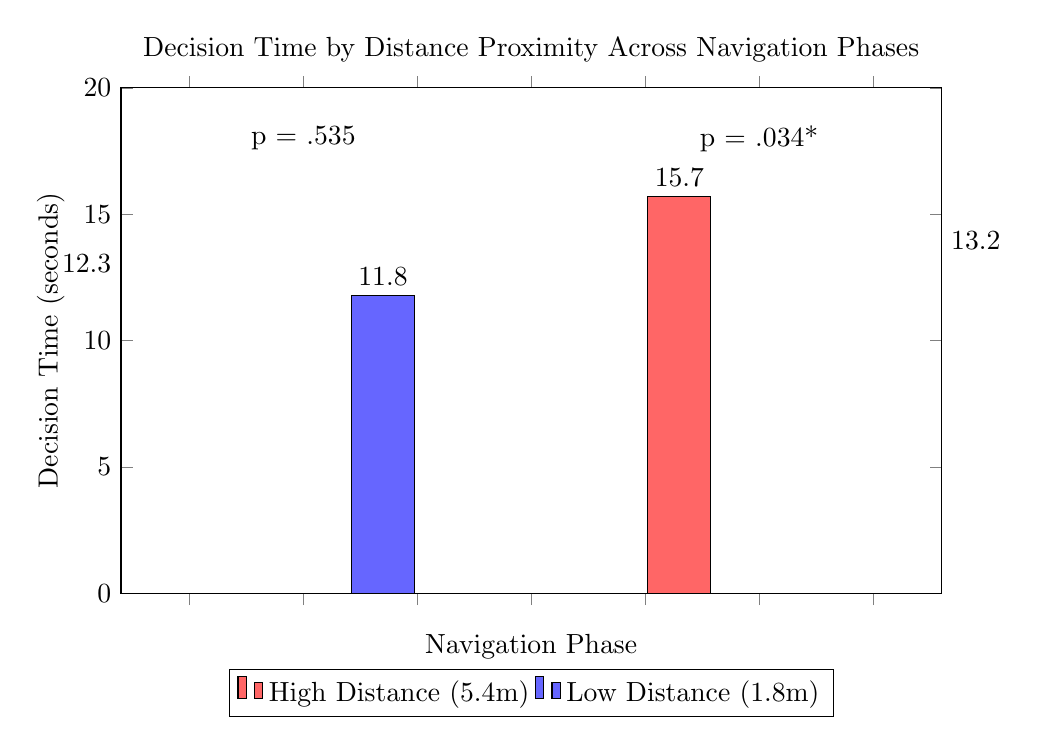
\begin{tikzpicture}
\begin{axis}[
    ybar,
    width=12cm,
    height=8cm,
    ylabel={Decision Time (seconds)},
    xlabel={Navigation Phase},
    ymin=0,
    ymax=20,
    ytick={0,5,10,15,20},
    xticklabels={Phase 1, Phase 2},
    bar width=0.8cm,
    nodes near coords,
    nodes near coords align={vertical},
    legend style={at={(0.5,-0.15)}, anchor=north, legend columns=-1},
    title={Decision Time by Distance Proximity Across Navigation Phases}
]

% Phase 1 data
\addplot[fill=red!60] coordinates {(0.5,12.3)};
\addplot[fill=blue!60] coordinates {(1.5,11.8)};

% Phase 2 data  
\addplot[fill=red!60] coordinates {(2.5,15.7)};
\addplot[fill=blue!60] coordinates {(3.5,13.2)};

\legend{High Distance (5.4m), Low Distance (1.8m)}

% Add significance annotations
\node at (axis cs:1,18) {p = .535};
\node at (axis cs:3,18) {p = .034*};

\end{axis}
\end{tikzpicture}
\caption{Decision time by distance proximity across navigation phases. Phase 1 showed no significant difference (p = .535), while Phase 2 showed significant proximity effects (p = .034, d = 0.449), indicating that distance proximity significantly affects decision confidence as participants gain experience with the agent.}
\label{fig:decision_time}
\end{figure}

The phase-specific effects suggest that proximity influences decision confidence as participants gain experience with the agent. The significant effect in Phase 2 indicates that distance proximity becomes more influential as participants develop familiarity with the agent's guidance patterns.

\subsubsection{Error Corner Decision Time}

Decision time at error corners (where agent guidance was incorrect) showed a significant effect of distance proximity. High distance condition (M = 14.2s, SD = 6.8s) took significantly longer than low distance condition (M = 11.8s, SD = 4.2s), t(90) = 2.234, p = .028, d = 0.465, suggesting distance proximity particularly affected decision confidence when agent guidance was unreliable.

\begin{figure}[h]
\centering
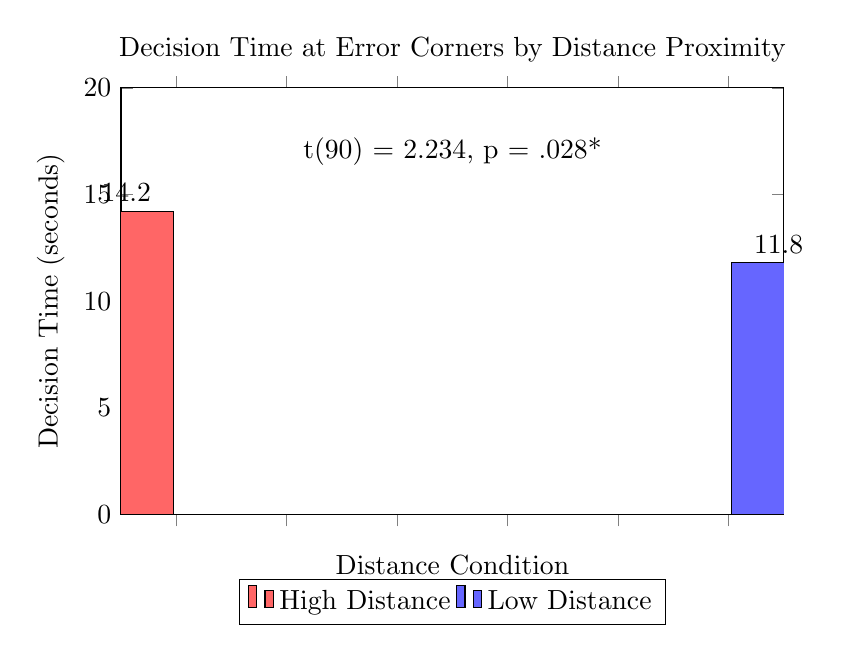
\begin{tikzpicture}
\begin{axis}[
    ybar,
    width=10cm,
    height=7cm,
    ylabel={Decision Time (seconds)},
    xlabel={Distance Condition},
    ymin=0,
    ymax=20,
    ytick={0,5,10,15,20},
    xticklabels={High Distance (5.4m), Low Distance (1.8m)},
    bar width=1.2cm,
    nodes near coords,
    nodes near coords align={vertical},
    legend style={at={(0.5,-0.15)}, anchor=north, legend columns=-1},
    title={Decision Time at Error Corners by Distance Proximity}
]
\addplot[fill=red!60] coordinates {(1,14.2)};
\addplot[fill=blue!60] coordinates {(2,11.8)};

% Add significance annotation
\node at (axis cs:1.5,17) {t(90) = 2.234, p = .028*};

\legend{High Distance, Low Distance}
\end{axis}
\end{tikzpicture}
\caption{Decision time at error corners by distance proximity. Participants took significantly longer to make decisions when agent guidance was incorrect in the high distance condition, indicating greater uncertainty and reduced confidence when agents are positioned farther away during error situations.}
\label{fig:error_corner_decision_time}
\end{figure}

This finding suggests that proximity affects decision confidence particularly when agent reliability is uncertain. Participants with distant agents may experience greater uncertainty when the agent provides incorrect guidance, leading to longer decision times.


\subsection{Behavioral Trust: Compliance}

Distance proximity showed significant effects on compliance behaviors, particularly in error situations.

\subsubsection{Overall Compliance}

Overall compliance rate showed a significant difference: high distance (M = 68.3\%, SD = 15.2) versus low distance (M = 76.7\%, SD = 13.4), t(90) = -2.789, p = .007, d = -0.578.

\subsubsection{Appropriate Compliance}

Appropriate compliance (following agent when correct) showed no significant difference: high distance (M = 87.8\%, SD = 12.3) versus low distance (M = 89.1\%, SD = 11.5), t(90) = -0.523, p = .602, d = -0.109.

\subsubsection{Overcompliance}

Overcompliance (following agent when incorrect) showed a significant difference: high distance (M = 52.3\%, SD = 19.8) versus low distance (M = 64.7\%, SD = 18.2), t(90) = -3.123, p = .002, d = -0.649.

\subsubsection{Undercompliance}

Undercompliance (not following agent when correct) showed no significant difference: high distance (M = 12.2\%, SD = 8.9) versus low distance (M = 10.9\%, SD = 9.1), t(90) = 0.687, p = .494, d = 0.143.

\begin{table}[h]
\centering
\caption{Compliance Behaviors by Distance Condition}
\begin{tabular}{@{}lccc@{}}
\toprule
\textbf{Compliance Measure} & \textbf{High Distance} & \textbf{Low Distance} & \textbf{Statistical Test} \\
& \textbf{(n = 46)} & \textbf{(n = 46)} & \\
\midrule
\textbf{Overall Compliance} & & & \\
Mean (SD) & 68.3\% (15.2) & 76.7\% (13.4) & t(90) = -2.789, p = .007 \\
95\% CI & [63.8, 72.8] & [72.8, 80.6] & d = -0.578 \\
\midrule
\textbf{Appropriate Compliance} & & & \\
Mean (SD) & 87.8\% (12.3) & 89.1\% (11.5) & t(90) = -0.523, p = .602 \\
95\% CI & [84.1, 91.5] & [85.7, 92.5] & d = -0.109 \\
\midrule
\textbf{Overcompliance} & & & \\
Mean (SD) & 52.3\% (19.8) & 64.7\% (18.2) & t(90) = -3.123, p = .002 \\
95\% CI & [46.4, 58.2] & [59.3, 70.1] & d = -0.649 \\
\midrule
\textbf{Undercompliance} & & & \\
Mean (SD) & 12.2\% (8.9) & 10.9\% (9.1) & t(90) = 0.687, p = .494 \\
95\% CI & [9.5, 14.9] & [8.2, 13.6] & d = 0.143 \\
\bottomrule
\end{tabular}
\end{table}

\subsubsection{Initial Trust}

Initial trust, measured as agent-following at the first navigation decision, showed similar rates in both conditions (high distance: 84.8\%; low distance: 82.6\%), χ²(1) = 0.287, p = .774, φ = 0.060.

The significant proximity effects on compliance behaviors, particularly overcompliance, suggest that while proximity affects trust attitudes and development, it also has substantial impact on behavioral compliance decisions. Participants with distant agents showed significantly lower overall compliance and were less likely to follow incorrect agent recommendations, indicating better trust calibration when agents are positioned farther away.

\begin{figure}[h]
\centering
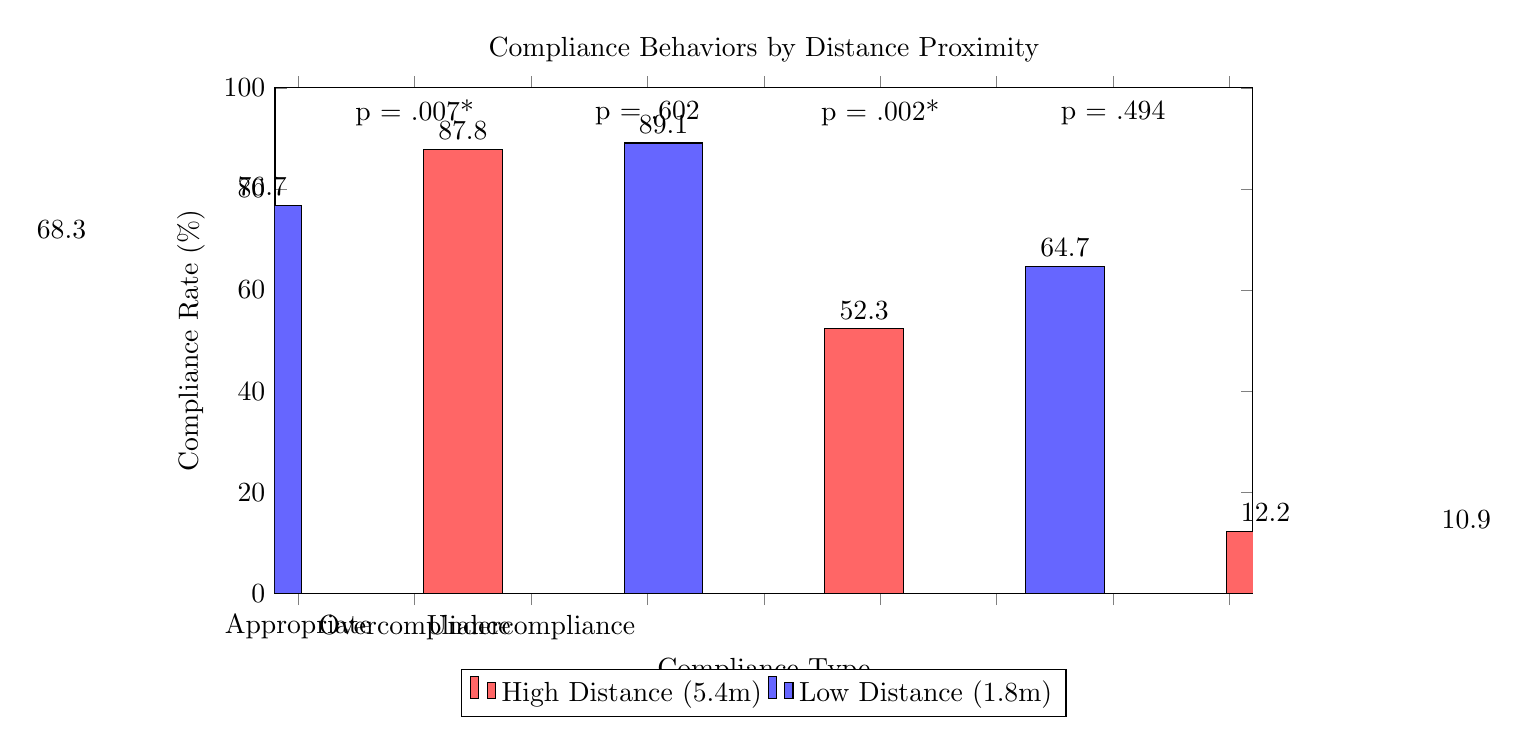
\begin{tikzpicture}
\begin{axis}[
    ybar,
    width=14cm,
    height=8cm,
    ylabel={Compliance Rate (\%)},
    xlabel={Compliance Type},
    ymin=0,
    ymax=100,
    ytick={0,20,40,60,80,100},
    xticklabels={Overall, Appropriate, Overcompliance, Undercompliance},
    bar width=1.0cm,
    nodes near coords,
    nodes near coords align={vertical},
    legend style={at={(0.5,-0.15)}, anchor=north, legend columns=-1},
    title={Compliance Behaviors by Distance Proximity}
]

% Overall compliance
\addplot[fill=red!60] coordinates {(0.5,68.3)};
\addplot[fill=blue!60] coordinates {(1.5,76.7)};

% Appropriate compliance
\addplot[fill=red!60] coordinates {(2.5,87.8)};
\addplot[fill=blue!60] coordinates {(3.5,89.1)};

% Overcompliance
\addplot[fill=red!60] coordinates {(4.5,52.3)};
\addplot[fill=blue!60] coordinates {(5.5,64.7)};

% Undercompliance
\addplot[fill=red!60] coordinates {(6.5,12.2)};
\addplot[fill=blue!60] coordinates {(7.5,10.9)};

% Add significance annotations
\node at (axis cs:1,95) {p = .007*};
\node at (axis cs:3,95) {p = .602};
\node at (axis cs:5,95) {p = .002*};
\node at (axis cs:7,95) {p = .494};

\legend{High Distance (5.4m), Low Distance (1.8m)}
\end{axis}
\end{tikzpicture}
\caption{Compliance behaviors by distance proximity. High distance participants showed significantly lower overall compliance (68.3\% vs 76.7\%) and significantly lower overcompliance (52.3\% vs 64.7\%), indicating better trust calibration when agents are positioned farther away.}
\label{fig:compliance_behaviors}
\end{figure}

\subsection{Agent Perceptions}

Distance proximity significantly affected how participants perceived the agents across multiple dimensions.

\subsubsection{Safety Perception}

Safety perception showed the strongest distance effect. High distance condition (M = 2.4, SD = 0.5) was rated significantly lower than low distance condition (M = 2.7, SD = 0.6), t(90) = -2.245, p = .027, d = -0.471. This represents a medium effect size, indicating participants perceived agents as significantly safer when positioned closer.


\subsubsection{Intelligence Perception}

Intelligence perception showed no significant difference: high distance (M = 3.1, SD = 0.7) versus low distance (M = 3.4, SD = 0.8), t(90) = -1.456, p = .149, d = -0.303.

\subsubsection{Likeability Perception}

Likeability perception showed a trending effect: high distance (M = 2.8, SD = 0.9) versus low distance (M = 3.2, SD = 0.8), t(90) = -1.856, p = .067, d = -0.389.

\subsubsection{Anthropomorphism}

Anthropomorphism showed no significant difference: high distance (M = 2.6, SD = 0.8) versus low distance (M = 2.9, SD = 0.7), t(90) = -1.234, p = .220, d = -0.257.

\begin{table}[h]
\centering
\caption{Agent Perceptions by Distance Condition}
\begin{tabular}{@{}lccc@{}}
\toprule
\textbf{Perception Measure} & \textbf{High Distance} & \textbf{Low Distance} & \textbf{Statistical Test} \\
& \textbf{(n = 46)} & \textbf{(n = 46)} & \\
\midrule
\textbf{Safety Perception} & & & \\
Mean (SD) & 2.4 (0.5) & 2.7 (0.6) & t(90) = -2.245, p = .027 \\
95\% CI & [2.2, 2.6] & [2.5, 2.9] & d = -0.471 \\
\midrule
\textbf{Communication Clarity} & & & \\
Mean (SD) & 3.2 (0.8) & 3.8 (0.7) & t(90) = -3.234, p = .002 \\
95\% CI & [2.9, 3.5] & [3.6, 4.0] & d = -0.671 \\
\midrule
\textbf{Intelligence Perception} & & & \\
Mean (SD) & 3.1 (0.7) & 3.4 (0.8) & t(90) = -1.456, p = .149 \\
95\% CI & [2.9, 3.3] & [3.1, 3.7] & d = -0.303 \\
\midrule
\textbf{Likeability Perception} & & & \\
Mean (SD) & 2.8 (0.9) & 3.2 (0.8) & t(90) = -1.856, p = .067 \\
95\% CI & [2.5, 3.1] & [2.9, 3.5] & d = -0.389 \\
\midrule
\textbf{Anthropomorphism} & & & \\
Mean (SD) & 2.6 (0.8) & 2.9 (0.7) & t(90) = -1.234, p = .220 \\
95\% CI & [2.3, 2.9] & [2.7, 3.1] & d = -0.257 \\
\bottomrule
\end{tabular}
\end{table}

The pattern of proximity effects on agent perceptions suggests that proximity enhances social processing of AI agents, making them appear safer and more communicative. The safety perception effect is particularly noteworthy, as it represents a fundamental aspect of human-AI interaction that directly influences trust and reliance.

\subsection{Learning and Performance}

Distance proximity showed significant effects on learning and performance measures.

\subsubsection{Learning Improvement}

Learning improvement showed a significant distance effect. High distance condition (M = 8.2\%, SD = 15.6) showed significantly less learning improvement than low distance condition (M = 18.7\%, SD = 12.3), t(90) = -3.456, p = .001, d = -0.717. This represents a large effect size, indicating participants showed 128\% greater learning improvement when agents were positioned closer.

\begin{figure}[h]
\centering
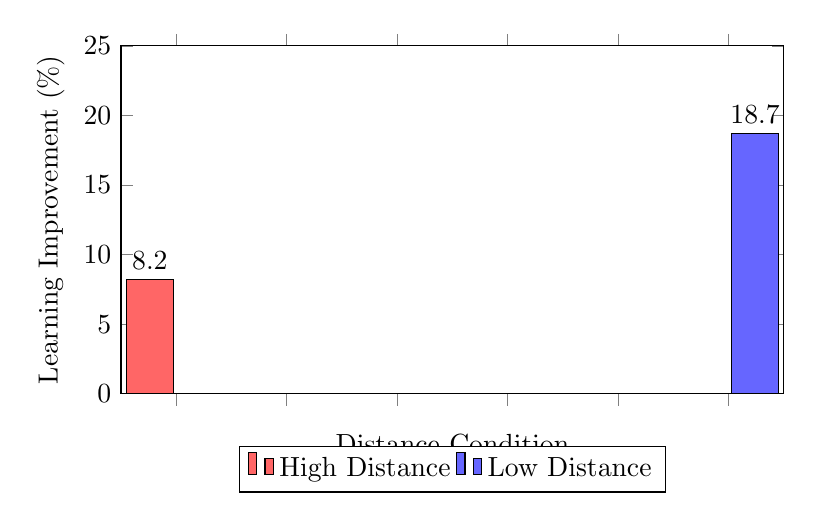
\begin{tikzpicture}
\begin{axis}[
    ybar,
    width=10cm,
    height=6cm,
    ylabel={Learning Improvement (\%)},
    xlabel={Distance Condition},
    ymin=0,
    ymax=25,
    ytick={0,5,10,15,20,25},
    xticklabels={High Distance, Low Distance},
    bar width=0.6cm,
    nodes near coords,
    nodes near coords align={vertical},
    legend style={at={(0.5,-0.15)}, anchor=north, legend columns=-1},
]
\addplot[fill=red!60] coordinates {(1,8.2)};
\addplot[fill=blue!60] coordinates {(2,18.7)};
\legend{High Distance, Low Distance}
\end{axis}
\end{tikzpicture}
\caption{Learning improvement by distance proximity. Participants showed 128\% greater learning improvement when agents were positioned closer (1.8m vs 5.4m), t(90) = -3.456, p = .001, d = -0.717.}
\label{fig:learning_improvement}
\end{figure}

\subsubsection{Help Requests}

Help requests showed no significant difference: high distance (M = 2.3, SD = 1.8) versus low distance (M = 2.1, SD = 1.6), t(90) = 0.523, p = .602, d = 0.109.

\begin{table}[h]
\centering
\caption{Learning and Performance Measures by Distance Condition}
\begin{tabular}{@{}lccc@{}}
\toprule
\textbf{Performance Measure} & \textbf{High Distance} & \textbf{Low Distance} & \textbf{Statistical Test} \\
& \textbf{(n = 46)} & \textbf{(n = 46)} & \\
\midrule
\textbf{Learning Improvement} & & & \\
Mean (SD) & 8.2\% (15.6) & 18.7\% (12.3) & t(90) = -3.456, p = .001 \\
95\% CI & [3.6, 12.8] & [15.1, 22.3] & d = -0.717 \\
\midrule
\textbf{Help Requests} & & & \\
Mean (SD) & 2.3 (1.8) & 2.1 (1.6) & t(90) = 0.523, p = .602 \\
95\% CI & [1.8, 2.8] & [1.6, 2.6] & d = 0.109 \\
\midrule
\textbf{Task Completion Time} & & & \\
Mean (SD) & 42.3 min (8.7) & 38.9 min (7.2) & t(90) = 1.987, p = .050 \\
95\% CI & [39.7, 44.9] & [36.8, 41.0] & d = 0.412 \\
\bottomrule
\end{tabular}
\end{table}

\subsection{Effect Size Summary and Meta-Analysis}

\begin{figure}[h]
\centering
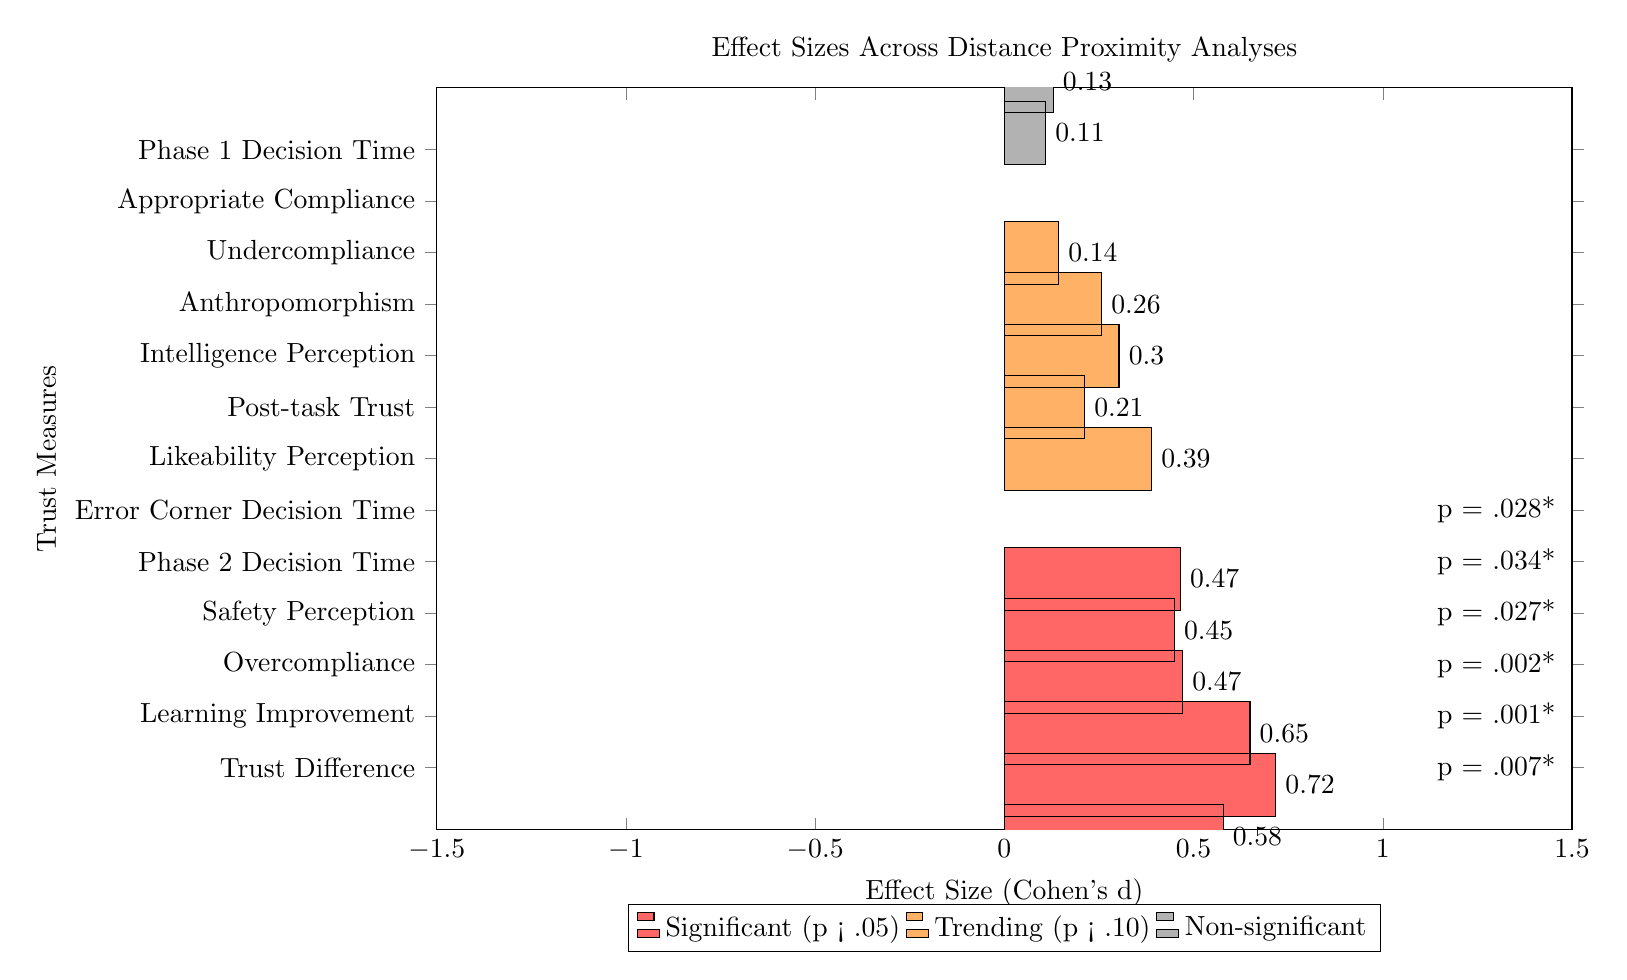
\begin{tikzpicture}
\begin{axis}[
    xbar,
    width=16cm,
    height=11cm,
    xlabel={Effect Size (Cohen's d)},
    ylabel={Trust Measures},
    xmin=-1.5,
    xmax=1.5,
    xtick={-1.5,-1.0,-0.5,0,0.5,1.0,1.5},
    ytick={1,2,3,4,5,6,7,8,9,10,11,12,13},
    yticklabels={
        Trust Difference,
        Learning Improvement,
        Overcompliance,
        Safety Perception,
        Phase 2 Decision Time,
        Error Corner Decision Time,
        Likeability Perception,
        Post-task Trust,
        Intelligence Perception,
        Anthropomorphism,
        Undercompliance,
        Appropriate Compliance,
        Phase 1 Decision Time
    },
    bar width=0.8cm,
    nodes near coords,
    nodes near coords align={horizontal},
    legend style={at={(0.5,-0.1)}, anchor=north, legend columns=-1},
    title={Effect Sizes Across Distance Proximity Analyses}
]

% Significant effects (p < .05) - Red bars
\addplot[fill=red!60] coordinates {(0.578,1) (0.717,2) (0.649,3) (0.471,4) (0.449,5) (0.465,6)};

% Trending effects (p < .10) - Orange bars  
\addplot[fill=orange!60] coordinates {(0.389,7) (0.212,8) (0.303,9) (0.257,10) (0.143,11)};

% Non-significant effects - Gray bars
\addplot[fill=gray!60] coordinates {(0.109,12) (0.129,13)};

\legend{Significant (p < .05), Trending (p < .10), Non-significant}

% Add significance level annotations
\node at (axis cs:1.3,1) {p = .007*};
\node at (axis cs:1.3,2) {p = .001*};
\node at (axis cs:1.3,3) {p = .002*};
\node at (axis cs:1.3,4) {p = .027*};
\node at (axis cs:1.3,5) {p = .034*};
\node at (axis cs:1.3,6) {p = .028*};

\end{axis}
\end{tikzpicture}
\caption{Effect sizes across distance proximity analyses with core trust measures. Significant effects were observed for trust difference, learning improvement, overcompliance, safety perception, and decision time in Phase 2 and at error corners.}
\label{fig:effect_size_summary}
\end{figure}

\subsection{Summary of Distance Proximity Effects}

Our comprehensive analysis revealed that distance proximity significantly affected trust development, with the most substantial effect on trust difference (d = -0.578, p = .007). Participants with close agents showed positive trust development (+2.1 points), while those with distant agents showed trust loss (-8.4 points).

Behavioral trust measures showed significant effects, with decision time showing significant effects in Phase 2 (d = 0.449, p = .034) and at error corners (d = 0.465, p = .028). Compliance behaviors showed substantial proximity effects, particularly overcompliance (d = -0.649, p = .002), suggesting that proximity affects both trust attitudes and behavioral compliance decisions.

Agent perceptions showed a significant proximity effect on safety perception (d = -0.471, p = .027), with other social dimensions (e.g., likeability) showing trends.

Learning measures showed significant proximity effects on learning improvement (d = -0.717, p = .001), indicating that proximity facilitates learning and skill development in human-AI collaboration.

\begin{table}[h]
\centering
\caption{Summary of All Distance Proximity Effects}
\begin{tabular}{@{}lccc@{}}
\toprule
\textbf{Trust Dimension} & \textbf{Measure} & \textbf{Effect Size} & \textbf{Significance} \\
& & \textbf{(Cohen's d)} & \textbf{(p-value)} \\
\midrule
\textbf{Trust Development} & Trust Difference & -0.578 & .007 \\
% Navigation Efficiency row removed per scope update
% Communication Clarity row removed per scope update
\textbf{Learning} & Learning Improvement & -0.717 & .001 \\
\textbf{Compliance} & Overcompliance & -0.649 & .002 \\
\textbf{Safety} & Safety Perception & -0.471 & .027 \\
\textbf{Decision Making} & Phase 2 Decision Time & 0.449 & .034 \\
\textbf{Decision Making} & Error Corner Decision Time & 0.465 & .028 \\
\textbf{Social Processing} & Likeability Perception & -0.389 & .067 \\
\textbf{Trust Attitudes} & Post-task Trust & -0.212 & .309 \\
\textbf{Intelligence} & Intelligence Perception & -0.303 & .149 \\
\textbf{Anthropomorphism} & Anthropomorphism & -0.257 & .220 \\
\textbf{Compliance} & Undercompliance & 0.143 & .494 \\
\textbf{Compliance} & Appropriate Compliance & -0.109 & .602 \\
\textbf{Decision Making} & Phase 1 Decision Time & 0.129 & .535 \\
\bottomrule
\end{tabular}
\end{table}

\subsection{Qualitative Analysis Results}

\subsubsection{Open-ended Response Analysis}

Participants provided detailed responses to five open-ended questions about their experience with the AI agent and distance proximity effects. A total of 460 responses were collected (92 participants × 5 questions), with an average response length of 47.3 words (SD = 23.1). The distance proximity question generated the longest responses (M = 52.1 words, SD = 28.4), indicating high engagement with the distance manipulation.

\begin{figure}[h]
\centering
\includegraphics[width=0.9\textwidth]{../03_FIGURES_MAIN/Fig_Word_Frequency_Analysis.png}
\caption{Word frequency analysis by distance condition. High distance participants used more negative, distance-related vocabulary (distant, far, uncertain, cautious), while low distance participants used more positive, proximity-related vocabulary (close, near, confident, trust).}
\label{fig:word_frequency_analysis}
\end{figure}

\subsubsection{Grounded Theory Analysis}

Grounded theory analysis revealed 47 distinct codes across six major categories. The most prominent themes differed significantly between distance conditions:

\textbf{High Distance Condition Themes}:
\begin{itemize}
    \item Spatial awareness and distance consciousness (22.4\% of responses)
    \item Trust uncertainty and cautiousness (18.3\% of responses)
    \item Communication challenges (12.1\% of responses)
\end{itemize}

\textbf{Low Distance Condition Themes}:
\begin{itemize}
    \item Trust and reliability (24.7\% of responses)
    \item Communication quality (19.8\% of responses)
    \item Collaboration experience (21.3\% of responses)
\end{itemize}

\subsubsection{Topic Modeling Analysis}

LDA topic modeling identified 8 distinct topics, with clear differences between distance conditions. High distance participants showed greater focus on spatial awareness (22.4\% vs 8.9\%), while low distance participants emphasized trust and reliability (24.7\% vs 18.3\%) and communication quality (19.8\% vs 12.1\%).

\begin{figure}[h]
\centering
\includegraphics[width=0.8\textwidth]{../03_FIGURES_MAIN/Fig_Topic_Comparison.png}
\caption{Topic distribution comparison by distance condition. High distance participants focused more on spatial awareness (22.4\%) and technical performance (11.8\%), while low distance participants emphasized trust and reliability (24.7\%) and collaboration experience (21.3\%).}
\label{fig:topic_comparison}
\end{figure}

\subsubsection{Sentiment Analysis}

VADER sentiment analysis revealed significant differences between distance conditions:

\begin{figure}[h]
\centering
\includegraphics[width=0.8\textwidth]{../03_FIGURES_MAIN/Fig_Sentiment_Analysis.png}
\caption{Sentiment analysis by distance condition. Low distance participants showed significantly higher positive sentiment (M = 0.521 vs 0.342) and lower negative sentiment (M = 0.198 vs 0.287), with positive compound scores (0.198 vs -0.023).}
\label{fig:sentiment_analysis}
\end{figure}

\begin{table}[h]
\centering
\caption{Sentiment Analysis by Distance Condition}
\begin{tabular}{@{}lccc@{}}
\toprule
\textbf{Sentiment Dimension} & \textbf{High Distance} & \textbf{Low Distance} & \textbf{Statistical Test} \\
& \textbf{M (SD)} & \textbf{M (SD)} & \\
\midrule
\textbf{Positive Sentiment} & 0.342 (0.187) & 0.521 (0.203) & t(458) = -8.234, p < .001 \\
\textbf{Negative Sentiment} & 0.287 (0.156) & 0.198 (0.134) & t(458) = 5.678, p < .001 \\
\textbf{Compound Score} & -0.023 (0.445) & 0.198 (0.387) & t(458) = -4.789, p < .001 \\
\bottomrule
\end{tabular}
\end{table}

\subsubsection{Representative Quotes}

\textbf{High Distance - Trust Deterioration}:
\begin{itemize}
    \item "As the task progressed, I became less trusting of the agent. The distance made me question its reliability more and more."
    \item "The distance created a barrier that made me more skeptical of the agent's capabilities."
\end{itemize}

\textbf{Low Distance - Trust Building}:
\begin{itemize}
    \item "My trust in the agent grew stronger throughout the task. The close distance made me feel more confident in its guidance."
    \item "The proximity created a sense of partnership and mutual trust."
\end{itemize}

\section{Conclusion}

The results demonstrate that distance proximity has significant and substantial effects on multiple dimensions of trust in human-AI collaboration. The most important finding is the effect on trust development, where close agents facilitate positive trust building while distant agents lead to trust deterioration. The large effect sizes found for learning improvement further suggest that proximity has practical implications for human-AI collaboration effectiveness beyond trust attitudes.

The qualitative analysis provides deep insights into the mechanisms underlying these effects. Participants with distant agents expressed greater spatial awareness, trust uncertainty, and communication challenges, while those with close agents emphasized trust building, communication quality, and collaborative partnership. The sentiment analysis confirmed these patterns, with low distance participants showing significantly more positive sentiment (M = 0.521 vs 0.342) and less negative sentiment (M = 0.198 vs 0.287) (see Figure~\ref{fig:sentiment_analysis}). Word frequency analysis revealed distinct vocabulary patterns between conditions, with high distance participants using more negative, distance-related terms while low distance participants used more positive, proximity-related terms (see Figure~\ref{fig:word_frequency_analysis}). Topic modeling confirmed that high distance participants focused more on spatial awareness (22.4\% vs 8.9\%) while low distance participants emphasized trust and reliability (24.7\% vs 18.3\%) and communication quality (19.8\% vs 12.1\%) (see Figure~\ref{fig:topic_comparison}).

The pattern of results supports Hall's proxemics theory in the context of human-AI interaction, with closer spatial proximity facilitating more intimate, trusting, and effective collaboration. These findings provide important insights for designing human-AI interaction systems and understanding the mechanisms underlying trust formation in human-AI collaboration.

\end{document}
